\chapter{Background and motivation}

We shall begin this paper by first looking into the already existing developments in the area of
asynchronous collaborative editing at the moment of our contact with the field. This chapter presents
the achievements and ideas of other researchers, with occasional comments regarding advantages or
disadvantages of the analyzed systems. In the end, we shall explain why we believed work in this
area was necessary and set as our objective to develop a new asynchronous editing system.

\section{Related work}

In this section we try to briefly introduce the reader to ongoing efforts in the area of asynchronous
collaborative editing and try to show the basis on which our work had to be built. We cover state-
as well as operation-based systems (see section \ref{sec:cmm} to find out more about the distinction
between the two types of systems) and discuss the ideas introduced in each of them.

\subsection{State-based version control systems}

The systems we present in this section are both widely-used, production systems and therefore we
relate more distantly to them than to the ones in the next section. However, they basically have
the same objectives that we do and therefore should be mentioned as related work.

\subsubsection{CVS}

CVS (Concurrent Versioning System) is the traditional versioning system used by programmers as aid for
collaborative source code development. Even though CVS can be used for collaborative editing of any
kind of text file, probably more than 90\% of the cases it is used for source code development. Virtually
everybody in the programming business has at least heard of CVS and most of us have also used it. Therefore,
we shall only give a brief description here as probably anything more than that would be common knowledge.
The information below comes from \cite{cvs}.

The Concurrent Versioning System implements a version control system: it keeps track of all work and all
changes in a set of documents, typically the implementation of a software project, and allows several
(potentially widely separated) developers to collaborate. CVS has become popular in the free software
world. Its developers release the system under the GNU General Public License.

CVS uses a client-server architecture: a server stores the current version(s) of the project and its
history, and clients connect to the server in order to check-out a complete copy of the project, work
on this copy and then later check-in their changes. Typically, client and server connect over a LAN
or over the Internet, but client and server may both run on the same machine if CVS has the task of
keeping track of the version history of a project with only local developers. The server software
normally runs on Unix, while CVS clients may run on any major operating-system platform.

Several clients may edit copies of the project concurrently. When they later check-in their changes,
the server attempts to merge them. If this fails, for instance because two clients attempted to change
the same line in a certain file, then the server denies the second check-in operation and informs the
client about the conflict, which the user will need to resolve by hand. If the check-in operation
succeeds, then the version numbers of all files involved automatically increment, and the CVS server
writes a user-supplied description line, the date and the author's name to its log files.

Clients can also compare different versions of files, request a complete history of changes, or
check-out a historical snapshot of the project as of a given date or as of a revision number. Many
open-source projects allow "anonymous read access", meaning that the clients may check-out and compare
versions without a password; only the check-in of changes requires a password in these scenarios.

Clients can also use the "update" command in order to bring their local copies up-to-date with the
newest version on the server. This eliminates the need for repeated downloading of the whole project.

CVS can also maintain different "branches" of a project. For instance, a released version of the
software project may form one branch, used for bug fixes, while a version under current development,
with major changes and new features, forms a separate branch.

The main advantages of CVS (which determined its wide-spread use from today) relate to the number of
facilities it offers to its users, such as version management, branch management, log management, project
structure management, security policies and many others which make it fit for use in production.
If it had not been for CVS, many of the open-source projects that exist today would not have been
possible to develop due to geographical separation of the developers. The open-source world owes
a lot to CVS.

However, the system also has several drawbacks, such as problems when renaming files, moving files to
a different directory, lack of proper support for binary files, limited security in sending passwords over the
network and so on. Other emerging systems (e.g. Subversion, BitKeeper) are trying to deal with these
problems and eventually build a better CVS.

The issue we are interested in from the perspective of our project is that CVS is a state-based versioning
control system, which bases its file comparison on the diff3 algorithm. The building block CVS works
with is the line. This means that the changes of two users are in conflict if they refer to the same
line. Concurrent changes that do not 'conflict', or touch the same lines of a file in different ways,
are merged automatically. Changes that do conflict are noted in the working files and sent back to the
user for manual resolution. It can, consequently, become very frustrating for the user, when merging
of changes cannot be done automatically, to manually analyze each conflict and decide what needs to
be kept and what needs to be removed. The fact that the only way to solve conflicts is by user
intervention is actually the problem with all state-based systems that exist today, not only CVS.

\subsubsection{Subversion}

The home page of Subversion (see \cite{subv}) gives the clearest comparison between it and CVS, which we
reproduce here in order to justify why this newer system is a step forward from CVS. Even though some
of the improvements are somewhat beyond the area of our discussion, we kept them for the sake of
completeness.

\begin{itemize}
\item \emph{Most current CVS features.}

Subversion is meant to be a better CVS, so it has most of CVS's features. Generally, Subversion's
interface to a particular feature is similar to CVS's, except where there's a compelling reason
to do otherwise.

\item \emph{Directories, renames, and file meta-data are versioned.}

Lack of these features is one of the most common complaints against CVS. Subversion versions not
only file contents and file existence, but also directories, copies, and renames. It also allows
arbitrary metadata ("properties") to be versioned along with any file or directory, and provides
a mechanism for versioning the `execute' permission flag on files.

\item \emph{Commits are truly atomic.}

No part of a commit takes effect until the entire commit has succeeded. Revision numbers are
per-commit, not per-file; log messages are attached to the revision, not stored redundantly as
in CVS.

\item \emph{Apache network server option, with WebDAV/DeltaV protocol.}

Subversion can use the HTTP-based WebDAV/DeltaV protocol for network communications, and the
Apache web server to provide repository-side network service. This gives Subversion an advantage
over CVS in interoperability, and provides various key features for free: authentication,
path-based authorization, wire compression, and basic repository browsing.

\item \emph{Stand-alone server option.}

Subversion also offers a stand-alone server option using a custom protocol (not everyone wants
to run Apache 2.x). The stand-alone server can run as an inetd service, or in daemon mode, and
offers basic authentication and authorization. It can also be tunneled over ssh.

\item \emph{Branching and tagging are cheap (constant time) operations.}

There is no reason for these operations to be expensive, so they aren't.

Branches and tags are both implemented in terms of an underlying "copy" operation. A copy takes
up a small, constant amount of space. Any copy is a tag; and if you start committing on a copy,
then it's a branch as well. (This does away with CVS's "branch-point tagging", by removing the
distinction that made branch-point tags necessary in the first place.)

\item \emph{Natively client/server, layered library design.}

Subversion is designed to be client/server from the beginning; thus avoiding some of the
maintenance problems which have plagued CVS. The code is structured as a set of modules
with well-defined interfaces, designed to be called by other applications.

\item \emph{Client/server protocol sends diffs in both directions.}

The network protocol uses bandwidth efficiently by transmitting diffs in both directions
whenever possible (CVS sends diffs from server to client, but not client to server).

\item \emph{Costs are proportional to change size, not data size.}

In general, the time required for an Subversion operation is proportional to the size of
the changes resulting from that operation, not to the absolute size of the project in
which the changes are taking place. This is a property of the Subversion repository model.

\item \emph{Efficient handling of binary files.}

Subversion is equally efficient on binary as on text files, because it uses a binary
diffing algorithm to transmit and store successive revisions.

\item \emph{Parsable output.}

All output of the Subversion command-line client is carefully designed to be both human
readable and automatically parsable; scriptability is a high priority.

\end{itemize}

The improvements we are mostly interested in are the fact that commits are truly atomic, that
the client/server protocol sends diffs in both directions and that costs are proportional to
change size, not to data size. Most of the rest are facilities our system does not deal with,
since it is only a prototype, not a production system (like CVS and Subversion are). This means
we were only interested in efficient, user-friendly, merging of versions and efficient bandwidth
use. The basic idea is that our system provides all of the three above mentioned as well (truly
atomic commits, diffs in both directions and costs proportional to changes), which means it
is, at least in these area, an improvement over CVS in the same way Subversion is.

The last thing to mention, however, is that \cite{subv} states that, currently, their merge support
is essentially the same as CVS's. This is where we tried to improve over Subversion as well and
create a merge support which is much more usable by the user.\\
\\
Beside CVS and Subversion, there are various other state-based systems which basically behave
more or less in the same way. Therefore, there is no point in talking about them anymore as we
would just be saying the same things all over again. Two examples of such other systems are
BitKeeper (see \cite{bitk}) and Microsoft Visual SourceSafe (see \cite{vss}).


\subsection{Operation-based version control systems}

The second category of systems we are going to discuss about are operation-based version control
systems. These are all still research systems (i.e. they still lack most of the facilities which
real users need in order to utilize them). However, they enclose very interesting ideas and, should
they be fit for commercial use, they would most likely find a lot of adopters. We relate more
closely to these projects both because our system is operation-based as well and because we have
also only developed a prototype system, not a fully-fledged production one.

\subsubsection{Safe Generic Data Synchronizer}

In \cite{molli03}, the authors propose using the operational transformation approach to define
a general algorithm for synchronizing a file system and file contents. The protocol they have
developed allows the use the same algorithm for synchronizing both the files of the file system
and the contents of those files. In order to achieve that, they propose a transformational approach
which is somewhat close to the one we used in our project.

The model of transformational approach considers $n$ sites. Each site has a copy of the shared
objects. When an object is modified on one site, the operation is executed immediately and sent
to others sites to be executed again. So every operation is processed in four steps: (a) generation
on one site, (b) broadcast to others sites, (c) reception by others sites, (d) execution on other
sites. The execution context of a received operation $op_i$ may be different from its generation
context. In this case, the integration of $op_i$ by others sites may leads to inconsistencies
between replicas. 

In the operational transformation approach, received operations are transformed according to
local concurrent operations and then executed. This transformation is done by calling
transformation functions. A transformation function $T$ takes two concurrent operations $op_1$ and
$op_2$ defined on the same state $s$ and returns $op'_{1}$. $op'_{1}$ is equivalent to $op_1$ but
defined on a state where $op_2$ has been applied.

The transformational approach defines two main components: \emph{the integration algorithm} and
\emph{the transformation functions}. The integration algorithm is responsible of receiving,
broadcasting and executing operations. It is independent of the type of shared data, it
calls transformation functions when needed. The transformation functions are responsible for
merging two concurrent operations defined on the same state. They are specific to the type
of shared data.

We are less interested in the generic algorithm they propose, since it is fit more closely
for real-time editing than for asynchronous editing. The idea that we want to underline, however, is that
of using transformation functions for integrating remote operations executed in different context.
We will apply the exact same idea in our project, with the distinction that we shall not address
the matter of file system synchronization, but only that of file content synchronization.

The main difference between the two approaches is that they use a fixed working unit, the so
called block while we use more flexible working units. Their operations are of the type addblock,
deleteblock and moveblock. The transformation functions are defined accordingly for each pair of
operations (addblock-addblock, addblock-delblock, addblock-moveblock, etc.). Our approach, on
the other hand, allows for far more granularity in what the working unit is concerned. This has
been on of our goals from the very beginning. We can work at paragraph, sentence, word or
character level as the blocks of our text documents. Moreover, our transformation functions do
not make any distinction between the levels of granularity. They work the same no matter whether
they deal with paragraphs, sentences, words or characters.

An earlier work of the same main authors (\cite{molli02}) relates in another way to our project,
namely in that it introduces transformation functions that work on trees. Their interest, however,
no longer lies in text editing, but in XML and CRC (Class, Responsibility, Collaboration) cards
editing (both of which types of documents are viewed as tree structures). The operations they
deal with here are CreateNode, DeleteNode, CreateAttribute, DeleteAttribute and ChangeAttribute.
Therefore, they need to define 25 transformation functions (for each pair of operations). The
paper describes, in essence, the same operation transformation mechanism as in the one mentioned
before. The distinction lies in the fact that the prototype described here also allows asynchronous
editing (however, details are not very abundant).

As we were saying, our interest with this paper comes from the use of tree operations. These are
fairly close to the ones we use in our model. The distinction comes from the fact that in
\cite{molli02} the logs of local operations are not distributed throughout the tree as in our
case. This means that the operations do determine changes to the tree structure, but they themselves
are kept separately from the structure of the tree, which means that still all remote operations
have to be transformed against all local operation, resulting in a performance loss.

A novel concept which is derived from using operations that work on trees is that the transformation
of an operation might lead to its cancellation (we refer to this as turning the operation into a
NOP (see \ref{sec:opdef})). We have used this concept in our project extensively as well.

\subsubsection{FORCE}

\cite{shen02} proposes a flexible merging framework in which semantic merging policies are separated
from the syntactic merging mechanism for asynchronous collaborative systems. In this framework,
semantic merging policies are not restricted by the merging algorithms used in the syntactic merging
mechanism, and the syntactic merging mechanism is flexible to support a wide range of semantic
merging policies. This framework is illustrated in figure \ref{fig:force}.

\begin{figure}[ht]
\begin{center}
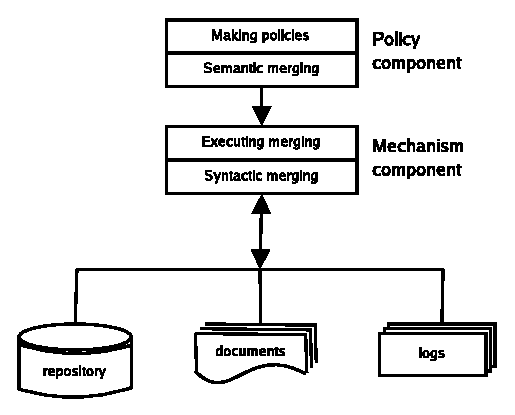
\includegraphics{img/force.eps}
\end{center}
\caption{The FORCE flexible merging framework}
\label{fig:force}
\end{figure}

\emph{The policy component} creates various semantic merging policies. These policies are
application-dependent. For example, if the shared document is an article, the semantic merging
policies could specify a set of spell and grammar checking rules. If the shared document is a
computer program, the semantic policies could specify the programming language's syntax parsing
rules. The essential observation is that if the work is properly divided among participants
in the way that different participants play different roles, it is possible that their concurrent
updates made to the shared document do not semantically conflict with each other, and therefore
a new document could be generated to integrate all the updates made by different participants.

\emph{The mechanism component} executes syntactic merging according to the policy specified in the
policy component. A remote update will be applied to a local working copy only if it does not
semantically conflict with any update performed by the local user according to the specified
policy. The mechanism component also includes some data structures: repository for storing versions,
logs for storing updates and document working copies. These data structures are needed for the
mechanism component to execute syntactic merging.

This is a very strong model which we have adopted ourselves. The policy component was kept fairly
simple and is represented by the semantic conflict function described in section \ref{sec:merge}.
We have also essentially adopted FORCE's basic merging algorithm (actually, adapted it to our
tree representation of the text document and, more importantly, distributed log). It best suited
our requirements since it uses operation-based merging and semantic rules for resolving conflicts.
However, in \cite{shen02}, the approach is described only for the linear representations of text
documents. The hierarchical representation that we have adopted in our approach yields a set of
advantages such as an increased efficiency and improvements in the editing semantics.

The way we used the algorithm described in FORCE will be explained in detail in later chapters.

\subsubsection{dARB}

Other researchers have also looked at tree representation of documents in the case of collaborative
editing. The dARB algorithm \cite{ion00} also uses a tree structure for representing the document,
however it is not able to automatically resolve all concurrent accesses to documents and, in some cases,
must resort to asking the users to manually resolve inconsistencies. They use an arbitration scheme for
resolving the conflicts in the case of real-time collaboration. The arbitration scheme decides to keep
the intentions of only one user in the case that some users perform concurrent operations that access
the same node in the tree. The arbitration is done according to priorities assigned to operation types.
For instance, the operations create/delete word (this is actually also an insert character operation, but
the inserted character is a space) are assigned a greater priority than the operation that modifies a
character in a word. There are cases when one site wins the arbitration and it needs to send not
only the state of the vertex itself, but maybe also the state of the parent or grandparent of the
vertex. For example, if one user performs a split of a sentence, while the other user concurrently
performs some modification in the original sentence, the user performing the split will win the
arbitration and need to send the state of the whole paragraph that contains the sentence to all other
users.

By allowing the customization of specifying the conflicts for various semantic units, our approach
is more general than the one defined in \cite{ion00} that considers that any concurrent operations
performed on the same vertex of a tree are conflicting. Moreover, their approach defines operations
(delete, insert) only at the character level in this algorithm, i.e. sending only one character at a
time, thus the number of packages through the network increases greatly. Our algorithm is not a
character-wise algorithm, but an element-wise one, i.e. it performs insertions/deletions of different
granularity levels (paragraphs, sentences, words and characters).

\subsubsection{Work in our group}

Last, but not least, we strongly relate our work to that done in our group in the previous years,
described in \cite{ignat02}, \cite{ignat03}, \cite{ignat04a}, \cite{ignat04b} and \cite{ned02}.
This work has been directed towards the development of a real-time collaborative text editing
based on a tree structure similar to the one we used in the current project. One of the goals of
our group is to integrate the two (now separate) editors into a single one where the user can choose
at any time if (s)he wants to work in an asynchronous manner or in a synchronous one.

The purpose of the project developed two years ago was to develop an efficient and reliable
concurrency control algorithm, and to implement a simple collaborative real-time editor relying
on this new algorithm.

Studying the existing algorithms constituted the first part of the project. Extensive testing which
include implementation of some of the algorithms was employed. This lead to the discovery of faults
in some of the algorithms. The entire process is described in detail in \cite{ned02}. The second
part of the project was concerned with the development and implementation of the algorithm itself,
aiming at maintaining not only the syntactic consistency, but also the semantic consistency. This
work was based on an already existing linear model, which, unfortunately, proved to be faulty in
some special cases. This, however, was only discovered towards the end of the project and the issue
has not yet been solved (neither by our group nor by other researchers).

The work presented in this paper comes as complementary to the one done two years ago, aiming to
contribute to achievement of the final goal of the group, namely to develop a universal information
platform that can support collaboration in a range of application domains such as engineering design
(CAD or CAAD) and collaborative writing (news agency, authoring of scientific papers or scientific
annotations), the basic unit for collaboration being the document. Since not all user groups have the
same conventions and not all tasks have the same requirements, this implies that it should be
possible to customize the collaborative editor at the level of both communities and individual
tasks \cite{ignat04b}.

\section{Motivation}

Collaborative editing systems have been developed to support a group of people editing documents
collaboratively over a computer network. The collaboration between users can be synchronous or
asynchronous. \emph{Synchronous collaboration} means that members of the group work at the same
time on the same documents and modifications are seen in real-time by the other members of the
group. \emph{Asynchronous collaboration} means that members of the group modify the copies of
the documents in isolation, afterwards synchronizing their copies to reestablish a common view
of the data.

Most existing systems either implement the synchronous mode of communication or the asynchronous
mode of communication, but not both of them. Since different user groups have different conventions
and requirements, software engineering as well other engineering domains require means of
customizing the collaborative work. An integrated system supporting both synchronous and
asynchronous collaboration is needed because these two modes of communication can be alternately
used in different stages of project development and under different circumstances. The real-time
feature is needed when the users in the team want to frequently interact to achieve a common
goal. The non-real-time feature is required if the users do not want to coordinate interactively
with each other. Also, the asynchronous mode of communication is useful in the case that
real-time collaboration cannot be performed for some period of time due to some temporary
failures, but can operate again afterwards.

In this line of thought, in order to contribute to the group's work towards achieving such a dual
system, we have taken upon ourselves the task of developing the module that deals with the asynchronous
mode of communication. What asynchronous editing means and the concepts involved will be discussed
in detail in chapter \ref{chap:concepts}, so we shall not cover them here. What we shall try to do
here instead is explain why the asynchronous editing mode is necessary and illustrate this with some
typical use cases.

\subsubsection{Hiding draft work from others}

One can easily imagine situations when users want to obtain a certain final version of their work
before showing it to others. There could be several reasons for wanting this, among which we could
mention:

\begin{itemize}
\item intermediate work might be incorrect. Think about a programmer working on an algorithm. It
      is obvious that most of the times the initial code (s)he writes is incorrect and should not
      be seen by the others. Under such circumstances, the author will probably prefer to develop
      and test the code first and only when (s)he thinks it is correct submit it to the repository.
\item intermediate work might be not make sense until it is complete. Think about the case when
      someone writes some paragraphs in a mixed order and decides to only rearrange them in the
      correct order at the end, when (s)he has written all of them. Until (s)he does that, someone
      else reading the paragraphs will be taken aback by the lack of logic. It is probably desirable
      to avoid that.
\item intermediate work might be just an attempt. If someone is not sure about adding something to
      a document, but starts writing it though with the intention of deciding whether to keep it
      or not later on (depending on the outcome), it would probably be best for others not to see
      this work until a decision to keep it has been made by its author.
\end{itemize}

By using asynchronous editing mode, authors can simply keep changing the document without the other
group members being able to see any of the modification and only commit it (make it available for
the other to see) only when it is complete.

\subsubsection{Increased efficiency}

In a vast majority of cases group members working together on a document each modify different parts
of it. The most obvious example is that of two or more authors working together on a book. Almost always
each author will work on his/her own chapters and not interfere with what the other authors are writing.
In such cases, it is common sense that it would make no sense to keep constantly synchronizing the
versions of the document when it is most likely that the modification would not even appear in the
part of the document the user is looking at/working on (only so much of a document can appear on the
computer screen at one time).

In such cases, it makes no sense to waste bandwidth and processing resources in order to achieve
something nobody really needs. Whenever one author needs to read something the other authors have
written, (s)he can simply update his/her version then and obtain the modifications. Aside from
bandwidth and processing power, this is also more efficient from the following point of view: when
somebody is writing something, it is very common that entire sections get deleted, modified, moved
around, rewritten and so on. If we were to use synchronous communication, all these actions would
be mirrored in all the documents on all sites. If, however, asynchronous communication is used,
a log compression method can be employed (see section \ref{sec:compress}) in order to cancel out
pairs of insert/delete operations that first insert and then delete the same thing. In this way,
a minimal set of operations which achieve the same effect can be sent over the network.

\subsubsection{Offline use}

Another reason for supporting asynchronous communication is for coming to the aid of dial-up users
(which, if we analyze statistics, represent way over 50\% of Internet users nowadays). When using
synchronous communication, there is no way in which users can work together without being connected
to the network, since communication between sites occurs constantly. This is no longer the case with
asynchronous editing, because the user him/herself gets to decide when communication is to take
place.

This way, the user can simply log to the Internet when (s)he wants to start working, check out the
current version of the document and then log off from the Internet and keep working without being
connected. After a certain period of time, the same user can re-log and commit his/her changes.
Asynchronous communication makes this possible. And there is certainly a lot of potential in this
given the large number of users which still use dial-up. Aside from that, there are also cases
when network failures might actually prevent all users from synchronizing with each other. This
would effectively render a synchronous editor unusable. However, asynchronous editing can go on
as if nothing had happened. The only problems that might arise would be delays in the transmission
of the changes, but there is no way to avoid this as long as the network is down.

Such a benefit is of even greater importance to the users who actually do not need to see what other
users are doing during the time in which they are working, as it would distract them. Take
programmers, for example: if someone is developing a stand-alone module which is to be used by
other then that someone will certainly not be interested in changes that others are making to
other functions, for instance. (S)he simply wants to focus on his/her work and submit it when it
is ready. Asynchronous communication is ideal for such style of work.

\subsubsection{Availability of changes history}

Asynchronous editing generally follows a client-server model. In this case, the server is known as
a repository, because it is where all the documents are kept. The essential difference between a
database server or a file server and a document repository of an asynchronous editing system is that
the repository stores not just the last version of the document, but actually all the versions
starting from the very first one. The advantage of such a system is that at any time any version
of the document can be retrieved and reviewed.

This is not the case with synchronous editors since in such systems there is usually no central
repository that stores all changes ever made to the document. The changes are only broadcast to
all sites that work together at one time and, at the end, just one final version is stored
(overwriting the old one). There are numerous cases, however, when old versions of the document
are needed, such as:

\begin{itemize}
\item in cases errors appear, older working versions represent a safety net one can fall on. This
      is especially common in software development where certain modifications can render parts of
      the (or even the entire) system unusable.
\item someone might want to find out (in an architecture project, for example) who was responsible
      for some ill decisions which might have lead to current problems.
\item coming back to software projects, it is often necessary to retrieve an older version of a
      program for example in order to install it on an older, less capable system.
\item there are cases when some parts of a document are deleted and the authors realize later that
      it would have been better to keep them. Since all intermediate versions are still available,
      it is fairly easy to find those deleted bits and reinsert them in the document.
\item version history is also useful for statistical purposes. Project managers frequently need to
      have an overview over the development of the project in order to make further decisions. Having
      an automated version history, it is relatively easy to obtain such an image of the evolution
      of the project.
\item various other cases when having access to older versions can be valuable.
\end{itemize}

It is hopefully clear that this is a great benefit which asynchronous systems alone can provide.\\
\\
Given what we have spoken about above, we hope that there is no further doubt in the mind of
the reader that efforts towards developing an asynchronous system are definitely not in vain.
Moreover, in addition to simply developing yet another asynchronous editing system, we have
strived (by analyzing what other before us have done, building upon their achievements and
learning from their mistakes) to actually come up with a system which would be valuable to
users also in terms of performance, not just in terms of what we have mentioned in this section.